%==========================
% Chapter 13: Production Systems and Synthesis
%==========================

\chapter{Production Systems and Synthesis}

\begin{keyinsight}
Training a model is only the beginning. Deploying it reliably in production requires understanding how information flows through the entire system: from user queries through retrieval, generation, validation, and monitoring. The principles that guided training---compression, uncertainty quantification, resource budgeting---apply equally to deployment. A production system is a model embedded in infrastructure, and both must be designed with information theory as the foundation.
\end{keyinsight}

\vspace{1.5em}

We have reached the final chapter of our journey from first principles to production systems. In Chapter 12, we explored how to train models at scale, balancing compute, parameters, and data according to scaling laws. Now we face a different challenge: taking that trained model and deploying it in an environment where queries arrive unpredictably, latency matters, failures must be handled gracefully, and costs accumulate with every request.

This chapter is about the gap between training and deployment. A model trained in a controlled environment with carefully curated data must now handle real users asking messy questions, expecting fast answers, and noticing when things go wrong. The infrastructure that serves the model must balance throughput and latency, manage limited GPU resources, monitor for drift, and respond to incidents.

But this is not just an engineering problem. It is an information-theoretic problem. Every deployment decision---how to quantize the model, which queries to cache, when to trigger retrieval, how to allocate GPU memory---is about managing information flow under constraints. The same principles that guided us through training continue to apply.

We will organize this chapter around three themes. First, we cover deployment essentials: the practical techniques for preparing models, serving them efficiently, monitoring their behavior, and responding to failures. Second, we walk through a complete case study of building a production RAG system, showing how the principles from Chapters 10, 11, and 12 come together in a real deployment. Third, we synthesize the entire book, showing how compression connects every chapter and distilling the principles that endure.

By the end of this chapter, you will understand not just how to deploy models, but why certain deployment patterns work. You will see that production systems are conversations between models and reality, mediated by infrastructure that must be designed with the same care as the models themselves. And you will have a framework for making deployment decisions grounded in information theory rather than folklore.

\vspace{2em}

%==========================
\section{Deployment Essentials}

%==========================

Deployment transforms a trained model into a system that serves real users. This transformation involves technical decisions about compression, infrastructure, monitoring, and failure handling. Each decision is a tradeoff, and understanding these tradeoffs requires thinking about information flow.

\begin{pausebox}[title=Deployment checklist (fast)]
\begin{itemize}
\item \textbf{Monitoring without ground truth.} When labels lag, combine proxy metrics (entropy, refusal rates, edit distance to previous versions) with spot-checked human audits. Active learning closes the loop: sample uncertain or drifting slices for labeling, retrain, and re-evaluate. Keep a small, frequently refreshed labeled canary set to detect regressions quickly.
\item \textbf{Testing and release hygiene.} Reliable launches pair unit tests for prompt templates and tools with integration tests for full pipelines (e.g., RAG with retrieval, reranking, and generation). Maintain a golden set for regression, property-based tests for invariants (schema validity, harmlessness), and adversarial suites for jailbreaks. Shadow traffic on new models catches surprising interactions before canary/blue-green rollout.
\end{itemize}
\end{pausebox}

\vspace{1em}

\begin{notationbox}
\textbf{Latency percentiles.} $p50/p95/p99$ denote the median and tail latencies. Users experience the tail: a system that is ``fast on average'' but slow at $p99$ feels broken.

\textbf{SLO vs.\ SLA.} An \emph{SLO} is your internal target (what you aim to meet). An \emph{SLA} is a customer-facing contract (what you must meet). Most teams design to an SLO with headroom so the SLA is rarely tested.

\textbf{Prefill vs.\ decode.} Transformer serving has a \emph{prefill} phase (process the prompt/context once) and a \emph{decode} phase (generate tokens one by one). The KV cache stores intermediate attention state so decode does not repeatedly recompute the full prompt.

\textbf{Confidence (as used here).} In this chapter, ``confidence'' means a \emph{system-level} estimate of correctness/answerability, ideally $c \approx P(\text{answer is correct} \mid q, \text{context}, a)$. The raw softmax probability of the generated text (or a model's self-reported ``confidence'') is not a reliable probability of correctness. In practice, teams learn $c$ from a small labeled canary set using a lightweight verifier or regressor over features (retrieval coverage, citation checks, self-consistency, log-prob). If you do not yet have labels, treat any confidence number as a proxy and use it conservatively for routing and abstention.
\end{notationbox}

\vspace{0.5em}

\subsection{Pre-Deployment: Model Preparation}

Before you serve a model, you must prepare it for production constraints. The model that achieved the best performance during training might be too large, too slow, or too memory-intensive for your deployment environment. Preparation means compressing the model without catastrophic quality loss.

\textbf{Quantization} reduces the precision of model weights and activations. A model trained in FP32 (32-bit floating point) uses 4 bytes per parameter. Quantizing to FP16 halves this to 2 bytes. Quantizing to INT8 reduces it to 1 byte, a 4$\times$ reduction. Quantizing to INT4 gives an 8$\times$ reduction but requires careful calibration to avoid quality loss.

From an information-theoretic perspective, quantization is lossy compression of the model itself. Each parameter is a continuous variable, and quantization discretizes it into a finite set of levels. Fewer levels mean less information capacity per parameter, which means the model can represent fewer distinct functions. The question is: how much precision can you discard before the model's outputs change significantly?

For most language models, FP16/BF16 causes negligible quality loss (often < 1\% increase in perplexity). \textbf{Caveat.} FP16/BF16 are not universally lossless; long-context arithmetic and exact string-match tasks can be sensitive because rounding error can compound across steps. Always measure.

INT8 quantization typically causes 1 to 3\% degradation if done carefully. INT4 can cause 5 to 10\% degradation but is still acceptable for some applications where speed and memory matter more than the last few percentage points of quality.

The key is to use post-training quantization or quantization-aware training. Post-training quantization converts a trained FP32 model to lower precision by finding optimal scales and zero-points for each layer. Quantization-aware training includes quantization in the training loop, so the model learns to be robust to precision loss. The latter yields better quality but requires retraining.

\textbf{Distillation} compresses a large "teacher" model into a smaller "student" model by training the student to mimic the teacher's outputs. Unlike quantization, which compresses representation, distillation compresses capacity. You trade model size for training cost: you spend more compute during training to produce a smaller model for inference.

Distillation works because the teacher provides soft targets (probability distributions over tokens) rather than hard labels (single correct tokens). These soft targets contain more information than hard labels: they tell the student not just which token is most likely, but how likely other tokens are. This richer signal helps the student learn faster and generalize better than training from scratch.

From a rate-distortion perspective, distillation is finding a lower-rate (smaller model) approximation to the teacher's distribution. The distortion (loss in quality) depends on how much you compress. A student with half the teacher's parameters might achieve 95\% of the teacher's performance. A student with one-tenth the parameters might achieve 85\%.

\textbf{Benchmarking} means measuring latency, throughput, and memory usage under realistic conditions before deploying. Do not trust theoretical estimates---measure on your actual hardware with your actual traffic patterns.

Latency has three components: time to load the model into GPU memory (happens once at startup), time to process the input (encode prompt, retrieve context), and time to generate the output (token by token). For a 7B parameter model on an A100 GPU, typical numbers are:

\vspace{0.5em}

\textbf{Startup latency:} 5 to 10 seconds to load weights

\textbf{Input processing:} 10 to 50 ms per 1,000 tokens (depends on batch size)

\textbf{Generation:} 20 to 100 ms per token (depends on batch size and sequence length)

\vspace{0.5em}

Throughput is measured in queries per second or tokens per second. A single A100 GPU can typically serve 10 to 50 queries per second for a 7B model, depending on whether you batch queries and how long the outputs are. Batching increases throughput but adds latency because queries wait for a batch to fill.

Memory usage has three components: model weights, key-value cache (for attention), and activations during generation. For a 7B parameter model in FP16, weights take 14 GB. The KV cache takes roughly 0.5 GB per 1,000 tokens of context \emph{per batch element}. Activations add a few GB. On an 80 GB A100, this typically fits comfortably at batch size $\sim$8 and context length $\sim$8{,}000 tokens; pushing to larger batches or longer contexts requires tradeoffs (paged attention, smaller batch, lower-precision KV cache, or a smaller model).

\vspace{1.5em}

\begin{examplebox}
\textbf{Quantization Tradeoffs: Concrete Numbers}

\vspace{0.5em}

Consider a 13B parameter model. In FP32, it requires 52 GB of memory just for weights (13B parameters $\times$ 4 bytes). This does not fit on a single 40 GB A100 GPU.

\vspace{0.5em}

\textbf{Option 1: FP16 quantization.} Reduces memory to 26 GB (13B $\times$ 2 bytes). Now it fits on one GPU with room for KV cache. Perplexity increases from 2.30 to 2.32 (< 1\% degradation). Inference is 1.5$\times$ faster due to FP16 tensor cores. \textbf{Cost:} Negligible quality loss. \textbf{Benefit:} Fits on one GPU, faster inference.

\vspace{0.5em}

\textbf{Option 2: INT8 quantization.} Reduces memory to 13 GB (13B $\times$ 1 byte). Perplexity increases to 2.38 (3.5\% degradation). Inference is 2$\times$ faster than FP16 because INT8 operations are faster. \textbf{Cost:} Noticeable but acceptable quality loss. \textbf{Benefit:} Can run on smaller GPUs (e.g., 24 GB consumer GPUs), twice the throughput.

\vspace{0.5em}

\textbf{Option 3: INT4 quantization.} Reduces memory to 6.5 GB. Perplexity increases to 2.55 (11\% degradation). Inference is 3$\times$ faster than FP16. \textbf{Cost:} Significant quality loss, unacceptable for most applications. \textbf{Benefit:} Can run on very small GPUs, very high throughput.

\vspace{0.5em}

\textbf{Decision:} For production serving where quality matters, use FP16. For high-throughput or resource-constrained environments where some quality loss is acceptable, use INT8. Reserve INT4 for specialized applications where speed dominates quality (e.g., on-device inference on mobile).
\end{examplebox}


\vspace{1.5em}

\subsection{Serving Infrastructure}

\vspace{0.3cm}
\textbf{Serving frameworks (selection heuristics).} If you need maximum throughput with long contexts and heavy KV-cache reuse, engines with paged attention and tensor parallelism are advantageous; for tight latency SLOs on many small requests, favor lightweight runtimes with aggressive batching and speculative decoding. Always report hardware, batch size, sequence lengths, and prompt/generation mix; raw QPS without these is meaningless.

\begin{pausebox}[title=Serving jargon (one page)]
\begin{itemize}
\item \textbf{KV cache.} The cached key/value tensors for attention. It grows with context length and batch size, and it often dominates serving memory.
\item \textbf{Prefill vs.\ decode.} Prefill processes the prompt once; decode generates tokens step-by-step. Many ``throughput'' bottlenecks are really decode bottlenecks.
\item \textbf{Paged attention.} A memory-management trick that stores KV cache in pages so long contexts and dynamic batching do not fragment GPU memory.
\item \textbf{Tensor parallelism.} Split a single model across multiple GPUs to fit larger models or speed up compute-heavy layers.
\item \textbf{Speculative decoding.} Use a small draft model to propose multiple tokens, then verify them with the large model to reduce decode latency.
\end{itemize}
\end{pausebox}

Once the model is prepared, you need infrastructure to serve it. Serving means accepting requests, running inference, and returning responses, all while managing resources efficiently.

\textbf{Serving frameworks} abstract away the low-level details of loading models, batching requests, and managing GPU memory. Popular options include:

\begin{itemize}
\item \textbf{vLLM:} Optimized for large language models, uses paged attention to maximize throughput. Good for high-volume serving.
\item \textbf{TensorRT-LLM:} NVIDIA's framework for optimizing transformer models. Compiles models for maximum performance on NVIDIA GPUs.
\item \textbf{TorchServe:} General-purpose PyTorch serving, good for rapid prototyping but less optimized than vLLM for LLMs.
\item \textbf{Text Generation Inference (TGI):} HuggingFace's serving framework, balances ease of use with performance.
\end{itemize}

The choice depends on your priorities. If you need maximum throughput and your model is a standard transformer, use vLLM. If you need custom model architectures or rapid iteration, use TorchServe. If you are already in the HuggingFace ecosystem, use TGI.

\textbf{Load balancing and autoscaling} distribute requests across multiple GPUs or machines. A single GPU can only handle so much traffic. When demand spikes, you need to add capacity dynamically.

Load balancing uses a proxy (e.g., NGINX, HAProxy, or a cloud load balancer) to route requests to backend servers running the model. The proxy tracks which backends are healthy, how loaded they are, and routes new requests to the least-loaded backend.

Autoscaling adds or removes backend servers based on metrics like queue length, average latency, or GPU utilization. When the queue grows beyond a threshold (e.g., 10 requests waiting), spin up a new instance. When the queue is empty for a sustained period (e.g., 5 minutes), spin down an instance to save cost.

The tradeoff is between responsiveness and cost. Aggressive autoscaling (low thresholds, fast spinup) keeps latency low but wastes money on idle capacity. Conservative autoscaling (high thresholds, slow spinup) minimizes cost but allows latency spikes during traffic surges.

A practical heuristic: set autoscaling thresholds so that p95 latency stays below your SLO (service level objective; internal target) during normal traffic, and p99 latency stays acceptable during 2$\times$ traffic surges. This usually means maintaining 20 to 40\% headroom: if your system can handle 100 queries per second, run enough instances to serve 120 to 140 QPS at baseline.

\textbf{GPU utilization} measures how effectively you use expensive GPU resources. A GPU sitting idle costs the same as a GPU running at full capacity, so high utilization is critical for cost efficiency.

Batching is the primary technique for improving utilization. Instead of processing one request at a time, accumulate a batch of requests and process them together. This amortizes the fixed costs of launching GPU kernels and memory transfers over multiple requests.

The tradeoff is latency versus throughput. Larger batches increase throughput (more queries per second) but increase latency for individual queries (they wait for the batch to fill). A batch size of 1 gives minimal latency but poor utilization. A batch size of 32 gives high utilization but adds tens of milliseconds of queueing delay.

Modern serving frameworks use dynamic batching: as requests arrive, accumulate them until either the batch reaches a size threshold (e.g., 16) or a time threshold (e.g., 10 ms) elapses, then process the batch. This balances latency and throughput adaptively.

\textbf{Cost estimation} is essential before deploying. How much will serving cost per query, per day, per month?

For cloud inference, costs are roughly:

\vspace{0.5em}

\textbf{GPU rental:} \$2 to \$8 per GPU-hour for on-demand A100s (often cheaper with reserved instances, spot, or pre-purchased capacity)

\textbf{Bandwidth:} \$0.05 to \$0.10 per GB egress (negligible for text, significant for images)

\textbf{Storage:} \$0.02 to \$0.05 per GB-month for model weights and logs

\vspace{0.5em}

A quick back-of-envelope starts from \emph{GPU-seconds per query}. A simple decomposition is:
\begin{equation}
t_{\text{query}} \approx t_{\text{prefill}}(T_{\text{in}}) + \frac{T_{\text{out}}}{\text{decode tok/s}}
\end{equation}
and the steady-state GPU count is roughly
\begin{equation}
N_{\text{GPU}} \approx \text{QPS} \times t_{\text{query}}.
\end{equation}

Example: if your effective decode speed is 50 tokens/second and you generate $T_{\text{out}} = 100$ tokens, decode alone costs $\sim$2 GPU-seconds per query. At 10 QPS sustained, that is $\sim$20 GPU-seconds per second, i.e., $\sim$20 GPUs \emph{if you serve with batch size 1 and no cache-aware optimizations}. In practice, dynamic batching, paged attention, and caching increase effective tokens/second and reduce the required GPUs by multiples. Quantization reduces cost primarily by increasing throughput and freeing memory (so you can batch more or hold longer contexts). The right number is workload-dependent---measure on your prompts and traffic.

\vspace{1em}


\subsection{Monitoring and Observability}

Production systems fail in unpredictable ways. Monitoring detects failures early, and observability helps diagnose root causes. The goal is to know when something is wrong before users notice, and to understand why it went wrong so you can fix it.

Recall from Chapter 11 that drift comes in three flavors: input drift, output quality drift, and calibration drift. In production, you monitor all three plus system health.

\textbf{Input drift} is detected by tracking the distribution of query embeddings over time. Compute embeddings of incoming queries using the same encoder you use for retrieval. Maintain a baseline distribution from training or early deployment, then monitor drift with a statistic that is robust in high dimensions (e.g., Mahalanobis distance with shrinkage/diagonal covariance, or PCA-reduced embeddings). Calibrate alert thresholds empirically (e.g., 99th/99.9th percentiles of the baseline) rather than using fixed numbers.

\textbf{Output quality drift} is harder to measure because you often lack ground truth labels for production queries. Use proxy signals:

\begin{itemize}
\item \textbf{Validation failures:} Track the rate at which generated outputs fail schema validation, range checks, or type checks. An increase signals degradation.
\item \textbf{Confidence proxies:} Track length-normalized entropy or log-prob of generated outputs. Shifts can flag distribution change, but these are weak proxies for correctness and should not be treated as ground truth.
\item \textbf{User feedback:} Track explicit feedback (thumbs up/down, query rephrases) as a direct signal of quality.
\item \textbf{A/B comparisons:} Maintain a reference model or cached responses, and randomly compare new outputs to reference outputs. Flag divergences for manual review.
\end{itemize}

\textbf{Calibration drift} is detected by binning predictions by confidence and tracking accuracy within bins. For generative models, true calibration requires at least a small labeled canary set (or a delayed-label pipeline). Separately, track \emph{stability} (e.g., self-consistency across samples) as a diagnostic signal; stability is not the same as calibration, but it can help surface regimes where uncertainty estimates are no longer meaningful.

\begin{pausebox}[title=When a drift alert fires (what to do)]
\begin{enumerate}
\item \textbf{Verify the alert.} Confirm the embedding model, preprocessing, and logging pipeline have not changed (false drift is common after a silent version bump).
\item \textbf{Slice the traffic.} Cluster queries (by topic or embedding) and identify which slices moved. ``Overall drift'' is rarely actionable; slice-level drift is.
\item \textbf{Localize the failure mode.} Is retrieval failing (low coverage / irrelevant docs), is generation changing (style, refusal rate), or is the system unhealthy (timeouts/OOMs)?
\item \textbf{Mitigate quickly.} Raise abstention thresholds, cap context length, reduce retrieval depth, or open a circuit breaker to a safer fallback while you diagnose.
\item \textbf{Fix and close the loop.} Update the index/corpus, fine-tune embeddings or rerankers, and refresh the labeled canary set so your confidence model stays calibrated.
\end{enumerate}
\end{pausebox}

\textbf{System health} metrics include:

\begin{itemize}
\item \textbf{Latency:} Track p50, p95, and p99 latency. Alert when your latency SLO is violated or when p99 spikes significantly.
\item \textbf{Throughput:} Track queries per second and tokens per second. Alert when throughput drops unexpectedly.
\item \textbf{Error rate:} Track HTTP 5xx errors, timeout errors, and out-of-memory errors. Alert when error rate exceeds 0.1 to 1\%.
\item \textbf{GPU utilization:} Track GPU memory usage and compute utilization. Alert when memory usage approaches limits (risk of OOM) or when utilization drops (waste of resources).
\item \textbf{Queue length:} Track the number of requests waiting for processing. Alert when queue length grows beyond capacity.
\end{itemize}

\textbf{Dashboard design} means choosing which metrics to display and what thresholds to use for alerts. A good dashboard answers three questions:

\begin{enumerate}
\item Is the system healthy right now? (Latency, error rate, throughput in the last 5 minutes)
\item Are there worrying trends? (Drift metrics, confidence scores, validation failures over the last 24 hours)
\item What happened during the last incident? (Historical view with drill-down to specific requests)
\end{enumerate}

A typical dashboard layout:

\vspace{0.5em}

\textbf{Top row:} Current status. Green if all metrics are within bounds, yellow if warnings, red if critical alerts.

\textbf{Second row:} Key metrics as time series over the last hour: latency (p50, p95, p99), throughput, error rate.

\textbf{Third row:} Drift and quality metrics over the last 24 hours: embedding drift distance, validation failure rate, average confidence.

\textbf{Bottom row:} System resources over the last hour: GPU utilization, memory usage, queue length.

\vspace{0.5em}

Do not overwhelm the dashboard with dozens of metrics. Choose 8 to 12 that matter most for your application, and make them large and visible. Use color (green/yellow/red) sparingly for critical alerts only.

\vspace{1em}


\subsection{A/B Testing and Measurement}

\vspace{0.3cm}
\textbf{A/B testing caveats.} The normal approximation breaks for small $n$ or extreme proportions; use exact or Bayesian tests in those regimes. Sequential designs (e.g., group-sequential or SPRT) allow peeking with error control. Correct for multiple comparisons (e.g., Bonferroni or FDR) when running many experiments. Skewed splits (e.g., 90/10) require \emph{larger} total samples for the same detectable effect. Latency and cost are often heavy-tailed; prefer quantile comparisons with bootstrap or nonparametric tests rather than assuming normality.
\textit{References:} Wald's \emph{Sequential Analysis} (1947) for SPRT; Benjamini--Hochberg (1995) for FDR control.

Before rolling out a new model or configuration to all users, test it on a subset. A/B testing splits traffic between a control (current system) and a treatment (new system), measures the difference in outcomes, and determines whether the treatment is better with statistical confidence.

\textbf{Experimental design} requires choosing three parameters: traffic split, duration, and success metric.

Traffic split determines what fraction of users see the treatment. Common splits are 50/50 (minimum total sample size for a fixed effect), 80/20 (common compromise), 90/10 (more conservative, limits exposure), or 95/5 (very conservative, used when the treatment is risky). The tradeoff is explicit: more conservative splits reduce risk but increase runtime because power drops.

Duration determines how long to run the experiment. Longer experiments give more data and higher confidence, but delay decision-making. Shorter experiments make faster decisions but risk false positives from noise. The duration depends on traffic volume and the size of the effect you expect.

A rule of thumb: run until you have at least 100 positive outcomes per group (e.g., 100 successful queries, 100 satisfied users). For low-traffic applications, this might take weeks. For high-traffic applications, a few hours suffice.

Success metric must align with what you care about. Accuracy is not enough if accuracy does not correlate with user satisfaction. Common metrics:

\begin{itemize}
\item \textbf{Task success rate:} Did the user accomplish their goal? (e.g., found the information they needed, completed the task)
\item \textbf{User satisfaction:} Explicit feedback (thumbs up/down) or implicit signals (time spent, query rephrases)
\item \textbf{Latency:} p95 or p99 latency (users care more about worst-case than average)
\item \textbf{Cost per query:} If you are optimizing for efficiency
\end{itemize}

The key is to measure what users experience, not just what the model does. A model with 2\% higher accuracy might have 5\% lower user satisfaction if the added accuracy comes at the cost of slower responses or more verbose outputs.

\textbf{Statistical significance} means determining whether the observed difference between control and treatment is real or due to random chance. Use a two-proportion z-test (for binary metrics like success rate). For heavy-tailed metrics like latency and cost, compare quantiles (p95/p99) with bootstrap confidence intervals or use nonparametric tests; a t-test on means can be misleading.

A common mistake is stopping the experiment as soon as you see significance. This introduces bias: you are more likely to stop when random fluctuations favor the treatment. Instead, either fix the duration in advance (based on power analysis) \emph{or} use a sequential design that makes peeking valid.

Power depends strongly on effect size and allocation. A 50/50 split minimizes total sample size; a 90/10 split typically needs $\sim$2--3$\times$ more total traffic for the same detectable effect under the same test assumptions.

\vspace{1.5em}

\begin{examplebox}
\textbf{A/B Test Design: Sample Size Calculation}

\vspace{0.5em}

Suppose you have a chatbot with 80\% task success rate. You deploy a new model that you believe will improve success rate to 85\%. How many users do you need to detect this 5\% improvement with confidence?

\vspace{0.5em}

Using standard power analysis for a two-proportion test:

\begin{itemize}
\item Baseline success rate: $p_1 = 0.80$
\item Treatment success rate: $p_2 = 0.85$ (hypothesized)
\item Significance level: $\alpha = 0.05$ (5\% false positive rate)
\item Power: $1 - \beta = 0.80$ (80\% chance of detecting the effect if it exists)
\end{itemize}

The required sample size per group is:

\begin{equation}
n = \frac{(z_{\alpha/2} + z_{1-\beta})^2 (p_1(1-p_1) + p_2(1-p_2))}{(p_2 - p_1)^2}
\end{equation}

where $z_{\alpha/2} = 1.96$ and $z_{1-\beta} = 0.84$ (80\% power).

\vspace{0.3em}

Plugging in:

\begin{align}
n &= \frac{(1.96 + 0.84)^2 (0.80 \cdot 0.20 + 0.85 \cdot 0.15)}{(0.85 - 0.80)^2} \\
  &= \frac{7.84 \cdot 0.2875}{0.0025} \\
  &\approx 902
\end{align}

\vspace{0.5em}

You need roughly 900 users per group, or 1,800 total. If your chatbot serves 1,000 users per day, run the experiment for 2 days. If it serves 10,000 users per day, a few hours suffice.

\vspace{0.5em}

If you use a 90/10 split instead of 50/50, you need \emph{more} total users for the same power. Under the same normal-approximation assumptions and effect size, you need roughly 4,600 total users (about 4,140 control and 460 treatment), i.e., $\sim$2.5$\times$ longer at the same traffic.
\end{examplebox}

\vspace{1.5em}


\subsection{Incident Response and Rollback}

Despite careful preparation, production systems fail. Models generate incorrect outputs, latency spikes, GPUs run out of memory, and infrastructure failures cascade. Incident response is about detecting failures quickly, mitigating impact, and recovering gracefully.

\textbf{Failure modes} in production LLM systems:

\begin{itemize}
\item \textbf{Model quality degradation:} The model starts producing low-quality outputs due to drift, contaminated data, or a bug in serving code.
\item \textbf{Latency spike:} Queries take much longer than usual due to long inputs, inefficient batching, or resource contention.
\item \textbf{Out-of-memory error:} GPU memory exhausted due to unexpectedly long contexts, memory leaks, or batch size misconfiguration.
\item \textbf{Cascading failure:} One component fails (e.g., retrieval service), causing upstream components to time out, overloading the entire system.
\item \textbf{Silent correctness failure:} The model returns plausible but incorrect outputs that validation does not catch, leading to user harm.
\end{itemize}

\textbf{Runbooks} are step-by-step procedures for responding to common incidents. A runbook for "latency spike" might look like:

\vspace{0.5em}

\textbf{1. Verify:} Check dashboard. Is p99 latency > 2$\times$ normal? Are multiple instances affected?

\textbf{2. Isolate:} Check recent deployments. Was there a config change or model update in the last hour?

\textbf{3. Mitigate:} If isolated to new instances, route traffic to old instances. If system-wide, increase autoscaling aggressiveness to add capacity.

\textbf{4. Diagnose:} Sample slow requests. Are they unusually long? Do they trigger expensive retrieval? Are they hitting a slow code path?

\textbf{5. Fix:} If due to config, roll back. If due to traffic pattern, add handling for long inputs (e.g., truncate or reject). If due to code, deploy hotfix.

\textbf{6. Monitor:} Watch latency for 1 hour after fix. If stable, resolve incident. If not, escalate.

\vspace{0.5em}

\textbf{Circuit breakers} prevent cascading failures by automatically disabling a failing component. For example, if the retrieval service is timing out on 50\% of requests, open the circuit: stop sending retrieval requests and fall back to generation without retrieval. This prevents the entire system from being dragged down by one failing component.

Circuit breakers have three states: closed (normal operation), open (failing component disabled), and half-open (testing whether component has recovered). Transitions:

\begin{itemize}
\item Closed $\to$ Open: If error rate exceeds threshold (e.g., 50\%) over a window (e.g., 10 requests).
\item Open $\to$ Half-open: After a timeout period (e.g., 30 seconds).
\item Half-open $\to$ Closed: If a test request succeeds.
\item Half-open $\to$ Open: If a test request fails.
\end{itemize}


\textbf{Rollback procedure} reverts to the previous stable version when a new deployment causes problems. The standard approach is blue-green deployment:

\begin{itemize}
\item \textbf{Blue environment:} Currently serving production traffic (e.g., model version 1.4).
\item \textbf{Green environment:} New version being deployed (e.g., model version 1.5).
\item Deploy to green, run tests, monitor metrics for a period (e.g., 10 minutes at 10\% traffic).
\item If green looks healthy, switch all traffic from blue to green.
\item If green has issues, keep traffic on blue and diagnose green offline.
\item Keep blue running for a grace period (e.g., 24 hours) to allow fast rollback if green has delayed failures.
\end{itemize}

This allows rollback in seconds: just route traffic back to blue. Compare this to in-place deployment, where rolling back requires redeploying the old version, which takes minutes or hours.

\textbf{Post-incident learning} means writing a postmortem that documents what happened, why it happened, and how to prevent recurrence. A good postmortem includes:

\begin{itemize}
\item Timeline of events (when was the incident detected, when was it mitigated, when was it resolved)
\item Root cause (the underlying reason, not just the proximate trigger)
\item Impact (how many users affected, for how long, what was the severity)
\item What went well (monitoring detected the issue quickly, runbook was effective)
\item What went poorly (alert was not clear, rollback took longer than expected)
\item Action items (concrete changes to prevent recurrence: add a new alert, improve validation, update runbook)
\end{itemize}

The goal is not to assign blame but to learn. Treat incidents as opportunities to improve the system.

\subsection{Security and Safety in Production}
\vspace{0.3cm}
Production systems defend against prompt injection, jailbreaks, and abuse with layered mitigations: input normalization and filtering, constrained tool schemas, and allowlisted function calls. For RAG, sanitize indexes (PII redaction) and attach provenance tags so downstream components can filter or down-rank untrusted sources. Model extraction and abuse risks are mitigated by rate limits, watermarking/API usage policies, and anomaly detection on query distributions. Document incident response: how to roll back models, revoke keys, and rotate credentials.

\vspace{1em}
\subsection{Privacy and Compliance}
\vspace{0.3cm}
Privacy programs include automated PII detection for both ingress and egress, documented retention policies, and auditable deletion workflows. For training on sensitive data, consider privacy-preserving techniques (e.g., sampling discipline, coarse aggregation); full differential privacy is possible but often degrades utility and requires care.

Production systems need PII detection (names, addresses, IDs) on ingress and egress; log only hashed or truncated content by default. Define retention windows; honor deletion requests (GDPR/CCPA) via versioned datasets and tombstoning. Keep an audit trail tying outputs to model+data+prompt versions, and use role-based access for raw logs.

\vspace{1em}
\subsection{Continuous Learning and Versioning}
\vspace{0.3cm}
Retraining cadence can be tied to drift signals and error audits. To mitigate catastrophic forgetting, teams use replay buffers, regularization toward previous parameters, or mixed-domain fine-tuning. Version \emph{model, data, prompts, retrieval corpora}, and \emph{tool schemas}. Progressive rollouts (shadow $\to$ canary $\to$ blue-green) provide rollback points. Prefer fine-tuning for small deltas; re-pretrain only when domain shifts invalidate base representations.

\vspace{1em}
\subsection{Multi-Model Routing and Cascades}
\vspace{0.3cm}
Difficulty/risk estimators for routing can be built from confidence proxies (entropy, margin), topic classifiers, or shallow performance predictors trained on past judgments. Cost--accuracy frontiers are traced by sweeping thresholds and plotting per-tier metrics; misroutes are audited and fed back into the router.

Route queries by estimated difficulty and risk. A common pattern: small model for the fast path, large model for hard cases, human fallback for critical or low-confidence. Log per-tier accuracy and latency; adjust thresholds to meet cost/SLO targets. Ensemble or mixture-of-experts setups require load-balancing and backpressure to avoid head-of-line blocking.

\vspace{1em}


\subsection{When Teams Should Not Use LLMs}
Prefer deterministic pipelines when inputs are structured and rules are stable. Retrieval-only or template-based systems often beat LLMs on latency, cost, and predictability for CRUD forms, CRUD APIs, and well-specified business rules. Use LLMs where ambiguity, open-ended text, or cross-domain generalization dominates.

\vspace{2em}

%==========================
\section{Integration Case Study: Building a Production RAG System}

\vspace{0.3cm}
\textbf{Editor's note (condensed).} To keep focus on decisions and outcomes, we omit low-level training minutiae (e.g., exact learning-rate schedules) and verbose diagrams here; a complete hyperparameter listing and system diagram are deferred to an appendix. We also clarify that this rapid (~3 months) delivery was feasible only because the team re-used existing engineering infrastructure (e.g., Kubernetes, logging, CI), had a narrow scope, and started with a clean dataset; first deployments in new domains typically take 6--12 months.
\vspace{0.3cm}
\textbf{Total cost of ownership.} GPU dollars are a small slice of cost. Data preparation, evaluations, and iteration typically dominate (e.g., two engineers over months \(\gg\) GPU spend). Timelines of 6--12 months are common for first deployments in new domains; compress only with existing infra and datasets.

%==========================

Let's put theory into practice. This section walks through a complete project from initial requirements to production deployment, showing how the principles from earlier chapters guide real decisions. The story is realistic: we encounter failures, make tradeoffs, and iterate. This is what building production AI actually looks like.

\vspace{1em}

\subsection{The Brief}

You are tasked with building an internal question-answering system for a mid-sized company (2,000 employees). The company has 100,000 internal documents: policies, technical documentation, project postmortems, and meeting notes. Employees waste hours searching for information. Your job is to make knowledge accessible.

\textbf{Requirements:}
\begin{itemize}
\item \textbf{Latency:} < 500 ms p95 (users will not wait longer)
\item \textbf{Task success:} > 90\% on a calibrated sample (thumbs-up is a proxy; you also run spot-checked human audits)
\item \textbf{Cost:} < \$2,000 per month (budget constraint)
\item \textbf{Timeline:} 3 months from kickoff to production
\end{itemize}

\textbf{Constraints:}
\begin{itemize}
\item Data is sensitive (internal documents cannot leave the company's infrastructure)
\item Team is small (you plus one engineer)
\item No prior LLM/RAG infrastructure (starting from scratch)
\end{itemize}

This is a classic RAG (retrieval-augmented generation) problem. You need to combine retrieval (find relevant documents) with generation (synthesize an answer). Let's walk through the phases.

\vspace{1em}

\subsection{Phase 1: Model Selection}

The first decision is which model to use. From Chapter 12, you know that compute-optimal training balances parameters and data, but you are not training from scratch---you are fine-tuning a pretrained model.

\textbf{Options considered:}

\begin{itemize}
\item \textbf{Large API model (GPT-4, Claude):} Highest quality, but costs \$0.01 to \$0.03 per request. At 10,000 queries per month, this is \$100 to \$300 per month---well within budget. But data must leave infrastructure (violates constraint). \textit{Rejected.}

\item \textbf{Self-hosted large model (70B parameters):} High quality, data stays internal. But typically requires multiple A100-class GPUs. Even at \$2 to \$8 per GPU-hour, 4$\times$ A100s costs \$5,840 to \$23,360 per month if run continuously. Far over budget. \textit{Rejected.}

\item \textbf{Self-hosted medium model (7B to 13B parameters):} Good quality, affordable. A 7B model can run on 1$\times$ A100; at \$2 per hour that is \$1,460 per month if run continuously. A 13B model may need 1--2 GPUs depending on precision and context length; at \$2 per hour that is \$1,460 to \$2,920 per month. \textit{Feasible with optimization.}

\item \textbf{Self-hosted small model (1B to 3B parameters):} Lower quality but cheap. Runs on consumer GPUs or small cloud instances. \textit{Backup option if budget is tight.}
\end{itemize}

\textbf{Decision:} Start with a 7B parameter model. Fine-tune on a sample of internal documents to adapt to the company's terminology and writing style. If quality is insufficient, scale up to 13B.

\textbf{Fine-tuning strategy:}

You have 100,000 documents (roughly 50 million tokens). Using the rough training-compute heuristic from Chapter 12, fine-tuning a 7B model on 50M tokens is on the order of $6 \times 7 \times 10^9 \times 50 \times 10^6 \approx 2.1 \times 10^{18}$ FLOPs. Converting FLOPs to wall-clock depends heavily on utilization; at an effective 30--100 TFLOP/s, this is roughly 6--20 GPU-hours on an A100. Either way, the dollar cost is small relative to engineering time and inference spend.

But you do not need to fine-tune on all 50M tokens. You curate a high-quality subset: 10,000 document-question pairs extracted from search logs and support tickets (and a small set written by subject-matter experts) and manually annotated. This is 5M tokens. A single fine-tuning run is on the order of 1--3 GPU-hours; you budget more wall-clock time for iteration and evaluation rather than raw compute.

\textbf{Training dynamics:}

Following Chapter 12, you design a learning rate schedule:
\begin{itemize}
\item Warmup: linear from $10^{-7}$ to $2 \times 10^{-5}$ over the first 5\% of steps
\item Stable: constant at $2 \times 10^{-5}$ for the next 80\% of steps
\item Decay: cosine decay from $2 \times 10^{-5}$ to 0 over the final 15\%
\end{itemize}

Batch size is 8 (limited by GPU memory with 2,048 token context). Use gradient accumulation with 4 steps to get effective batch size 32.

\textbf{Result:}

Pretrained model: perplexity 12.3 on held-out company documents

Fine-tuned model: perplexity 8.1 on held-out company documents

The 33\% reduction in perplexity suggests the model has adapted to the company's domain. You test on 100 curated questions and find 78\% accuracy (model gives correct answer in the top response). This is below the 90\% target, but you have not yet added retrieval.

\vspace{1em}

\subsection{Phase 2: System Design}

Now you design the full RAG system. From Chapter 11, you know the four-stage pattern: Encode, Budget, Verify, Act. Let's apply it.

\textbf{Stage 1: Encode.}

User submits a question. You encode it into an embedding using the same encoder used to embed documents. You also parse the question to identify intent (e.g., policy question, technical question, historical question) using a lightweight classifier.

\textbf{Stage 2: Budget.}

Based on intent and a cheap \emph{answerability} estimate, decide whether to retrieve and how much. For common, well-covered policy questions where the router predicts retrieval will not help, you can skip retrieval. For specific questions (entities, incidents, technical details) or when answerability is low, retrieve a larger candidate set (e.g., top 20) with hybrid search, then rerank down to the top 5.

Hybrid search (from Chapter 11) combines BM25 (keyword matching) with embedding similarity. Because these scores live on different scales, normalize each component per query before mixing:
\begin{equation}
\text{score}(q, d) = 0.7 \cdot \tilde{s}_{\text{emb}}(q, d) + 0.3 \cdot \tilde{s}_{\text{BM25}}(q, d)
\end{equation}

Here $\tilde{s}_{\text{emb}}$ and $\tilde{s}_{\text{BM25}}$ are per-query normalized scores (e.g., min-max over candidates). BM25 catches queries with specific entity names or technical terms. Embeddings catch semantic similarity. The 0.7/0.3 weighting is tuned empirically on a validation set.

Min-max normalization is a reasonable baseline, but it can be brittle when a single outlier dominates the candidate set. In production, rank-based normalization (mixing ranks rather than raw scores) or z-scoring over the retrieved candidates is often more stable. Whatever you choose, treat the mixing weight as a parameter: tune it on a held-out retrieval set (e.g., maximize recall@20 or nDCG) and re-tune after major corpus or embedding changes.

After retrieving 20 candidates with hybrid search, rerank using a cross-encoder (a BERT-style model that scores query-document pairs). Keep top 5 after reranking. This two-stage retrieval improves precision: instead of 60\% of top-5 documents being relevant (with single-stage), 85\% are relevant (with reranking).

\textbf{Stage 3: Verify.}

The model generates an answer. You verify:
\begin{itemize}
\item Schema check: Is the output valid JSON with required fields (answer, confidence, sources)?
\item Length check: Is the answer between 20 and 500 characters? (Reject too short or too long)
\item Citation check: Are all cited sources in the retrieval set? (Prevents hallucinated citations)
\item Abstention threshold: Is the system-level confidence score above your threshold? (If not, abstain rather than guess. Use stricter thresholds for high-risk/factual queries.)
\end{itemize}

If verification fails, trigger fallback: re-ask with additional constraints or abstain with a message: "I couldn't find a confident answer. Here are the most relevant documents: [links]."

\textbf{Stage 4: Act.}

Return the answer to the user. Log the query, retrieval results, generated answer, and user feedback (thumbs up/down) for monitoring.

\textbf{Architecture diagram (schematic):}

\usetikzlibrary{positioning}
\begin{center}
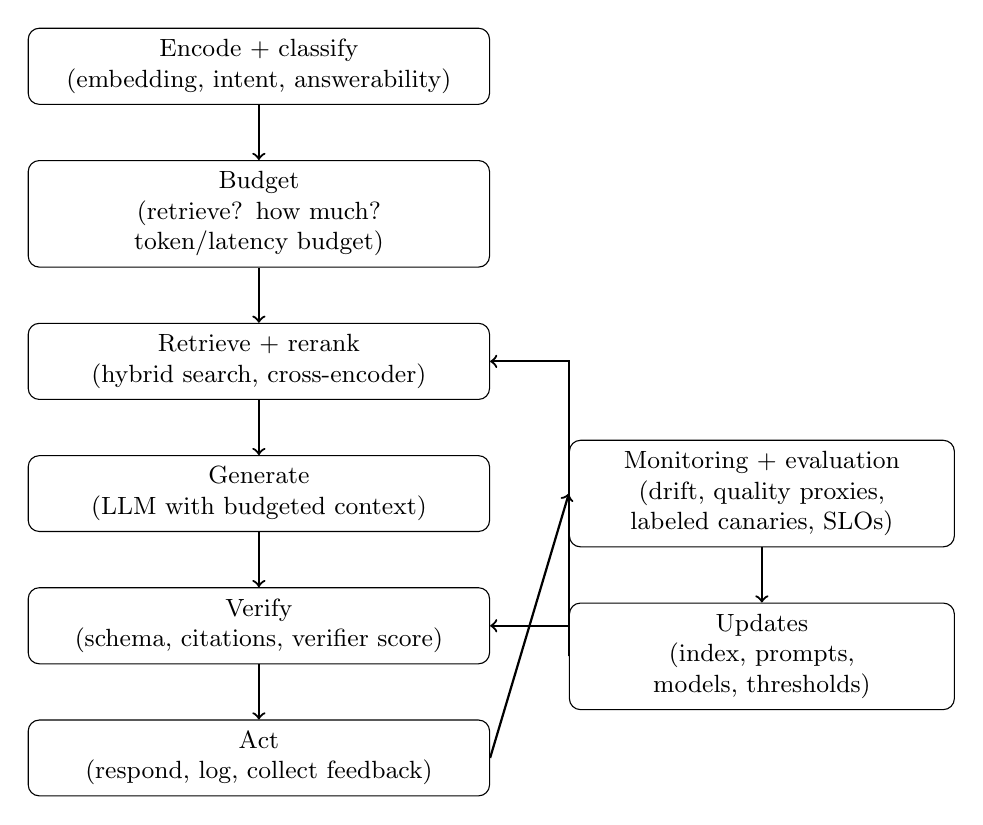
\begin{tikzpicture}[
  font=\small,
  node distance=7mm,
  box/.style={draw, rounded corners, align=center, inner sep=4pt, text width=0.46\linewidth},
  side/.style={draw, rounded corners, align=center, inner sep=4pt, text width=0.38\linewidth},
  arrow/.style={->, thick},
]
  \node[box] (encode) {Encode + classify\\(embedding, intent, answerability)};
  \node[box, below=of encode] (budget) {Budget\\(retrieve? how much?\\token/latency budget)};
  \node[box, below=of budget] (retrieve) {Retrieve + rerank\\(hybrid search, cross-encoder)};
  \node[box, below=of retrieve] (generate) {Generate\\(LLM with budgeted context)};
  \node[box, below=of generate] (verify) {Verify\\(schema, citations, verifier score)};
  \node[box, below=of verify] (act) {Act\\(respond, log, collect feedback)};

  \draw[arrow] (encode) -- (budget);
  \draw[arrow] (budget) -- (retrieve);
  \draw[arrow] (retrieve) -- (generate);
  \draw[arrow] (generate) -- (verify);
  \draw[arrow] (verify) -- (act);

  \node[side, right=10mm of generate] (monitor) {Monitoring + evaluation\\(drift, quality proxies,\\labeled canaries, SLOs)};
  \node[side, below=of monitor] (update) {Updates\\(index, prompts,\\models, thresholds)};

  \draw[arrow] (act.east) -- (monitor.west);
  \draw[arrow] (monitor) -- (update);
  \draw[arrow] (update.west) |- (retrieve.east);
  \draw[arrow] (update.west) |- (verify.east);
\end{tikzpicture}
\end{center}

\textbf{Monitoring (from Chapter 11):}

Track three signals:
\begin{itemize}
\item Input drift: Embedding drift over time (alert if drift score exceeds a calibrated threshold, e.g., above the baseline 99.5th percentile)
\item Output quality: Validation failure rate (alert if > 5\%) and user feedback (alert if thumbs-down rate > 20\%)
\item System health: p95 latency (alert if > 500 ms p95 SLO), throughput, error rate
\end{itemize}

\vspace{1em}

\subsection{Phase 3: Deployment}

You deploy on a small Kubernetes cluster with 1$\times$ A100 GPU for the 7B generator. Retrieval runs on CPU, and the reranker is small enough to serve on CPU at this traffic level, keeping the system within budget.

\textbf{Infrastructure choices:}

\begin{itemize}
\item \textbf{Serving framework:} vLLM for the generator (optimized for throughput), TorchServe for the reranker (CPU-served cross-encoder)
\item \textbf{Vector store:} FAISS for embedding search (fast, runs in-memory, handles 100K documents easily)
\item \textbf{Monitoring:} Prometheus for metrics collection, Grafana for dashboards
\item \textbf{Load balancer:} NGINX (simple, sufficient for internal tool with 2,000 users)
\end{itemize}

\textbf{A/B test:}

Before rolling out to all users, run an A/B test with 10\% of traffic (200 users) for 1 week. Compare new RAG system (treatment) to existing keyword search (control).

\textbf{Results after 1 week:}

\begin{center}
\begin{tabular}{lcc}
\textbf{Metric} & \textbf{Control (keyword search)} & \textbf{Treatment (RAG)} \\
\hline
Task success rate & 62\% & 87\% \\
Thumbs up rate & 45\% & 82\% \\
p95 latency & 120 ms & 420 ms \\
Cost per query & \$0.001 & \$0.15 \\
\end{tabular}
\end{center}

The RAG system dramatically improves accuracy and satisfaction, but it is slower (420 ms vs 120 ms, though still within the 500 ms p95 SLO) and about 150$\times$ more expensive per query. The higher cost is acceptable because the monthly budget (\$2,000) accommodates 13,000 queries, and usage is only 10,000 queries per month.

\textbf{Rollout:}

After the A/B test, you roll out to 50\% of users for 3 days, monitor metrics, then roll out to 100\%. The rollout is smooth: no incidents, latency remains below 500 ms p95, and user feedback is strongly positive (85\% thumbs up).

\textbf{Final production numbers:}

\begin{itemize}
\item Task success: 92\% (measured by thumbs-up on an audited sample)
\item Latency: 380 ms p50, 470 ms p95, 620 ms p99 (meets the 500 ms p95 SLO; p99 is higher, which you accept for now)
\item Cost: \$1,850 per month (1$\times$ A100 GPU + storage + bandwidth)
\item Serving: 10,000 queries per month, peak 20 queries per minute
\end{itemize}

You have met all requirements: > 90\% accuracy, < 500 ms p95 latency, < \$2,000 monthly cost. The project ships on schedule.

\vspace{1em}

\subsection{Iteration and Learning}

The first deployment is not perfect. Over the next two months, you encounter failures and iterate.

\textbf{Failure 1: Low retrieval quality}

In the first week, you notice that 15\% of thumbs-down responses cite "irrelevant retrieved documents." Upon inspection, you find that the initial embedding model (a general-purpose sentence-transformer) does not understand company-specific jargon. "KRI" (a company-specific term for Key Result Indicator) does not match queries about "key results."

\textbf{Fix:} Fine-tune the embedding model on company documents. You create a small training set of 5,000 query-document pairs labeled as relevant or irrelevant. Fine-tuning takes 2 GPU-hours and costs \$4. The new embeddings improve retrieval precision from 85\% to 92\%.

\textbf{Lesson:} Retrieval quality was the bottleneck, not model size. You could have used a smaller generator (3B instead of 7B) and invested more in retrieval. This would have reduced cost and latency while maintaining quality.

\textbf{Failure 2: Low cache hit rate}

You expected 40\% of queries to be duplicates or near-duplicates, allowing you to cache answers. Actual cache hit rate is 12\%. Why? Users phrase questions differently even when asking about the same topic.

\textbf{Fix:} Implement semantic caching. Instead of caching exact queries, cache embeddings. When a new query arrives, check if its embedding has cosine similarity $\ge 0.95$ to any cached query (equivalently cosine distance $\le 0.05$). If so, return the cached answer. This increases cache hit rate to 35\%, reducing average latency from 420 ms to 320 ms.

\textbf{Lesson:} Caching strategy must account for semantic similarity, not just string matching. This is an application of the information-theoretic principle from Chapter 11: caching exploits redundancy in the query distribution.

\textbf{Failure 3: Edge cases with no confident answer}

Some queries are unanswerable from the knowledge base (e.g., "What is the Wi-Fi password for the guest network?" when this is not documented). The model generates plausible but incorrect answers that pass schema checks and look ``confident'' under naive proxies (fluent text, low entropy). Validation does not catch these because they are syntactically valid.

\textbf{Fix:} Add a stricter abstention threshold for factual questions. Train (and periodically recalibrate) a lightweight verifier to estimate $c \approx P(\text{correct}\mid q,\text{retrieved},a)$ on a labeled canary set, then abstain when $c < 0.7$ for factual queries (opinion/discussion questions can tolerate lower thresholds). Return: "I don't have a confident answer. You might try asking [person responsible for this area]."

Additionally, you add a feedback loop: users can mark answers as incorrect. These flagged queries are reviewed monthly, and if a pattern emerges (e.g., many unanswerable questions about a topic), you add explicit handling or update the knowledge base.

\textbf{Lesson:} Validation must be task-specific. Generic schema checks are not enough. You need domain-specific rules and human-in-the-loop feedback.

\textbf{Success: Monitoring catches drift before users do}

Three months after launch, your drift detector alerts that the drift score has exceeded its calibrated threshold (e.g., above the 99.9th percentile of baseline). You inspect recent queries and find a spike in questions about a new product launch. The knowledge base does not yet include documentation for this product, so retrieval fails and the model guesses.

You quickly add product documentation to the knowledge base, re-index, and the drift alert clears. Users did not notice the issue because you caught it early.

\textbf{Lesson:} Monitoring works. The investment in drift detection (Chapter 11) pays off by catching issues before they become user-facing failures.

\vspace{1em}

\subsection{Lessons}
\begin{itemize}
\item \textbf{Data quality dominates.} Most downstream issues reduced to missing/ambiguous context; retrieval and schema validation paid for themselves.
\item \textbf{Budget early, validate always.} Token/cost budgets and confidence thresholds---decided upfront---avoided later rework.
\item \textbf{Measure what you deploy.} Latency/cost/quality dashboards and drift monitors turned surprises into routine maintenance.
\end{itemize}
\section{Synthesis: The Information Thread}
%==========================

We have traveled from first principles to production systems. It is time to step back and see the unified picture. Every chapter in this book is connected by a single idea: \textbf{learning is compression, and intelligence emerges from compressing the structure of the world into efficient representations}.

\vspace{1em}


\subsection{Revisiting Every Chapter Through Compression}

Let's trace the thread from Chapter 1 to Chapter 13, showing how compression unifies everything.

\textbf{Chapter 1: Learning is compression.}

We began with the fundamental insight: a good model compresses data. The better you compress, the better you understand. Cross-entropy measures average codelength, and minimizing it is equivalent to maximizing likelihood. Compression and learning are the same process viewed through different lenses.

From this foundation, everything else follows. If learning is compression, then:
\begin{itemize}
\item Regularization is preventing the model from using more bits than necessary (MDL principle).
\item Generalization is compressing not just the training data but the underlying distribution (compression implies prediction).
\item Evaluation is measuring how efficiently the model encodes test data (cross-entropy is bits per token; perplexity is its exponentiation).
\end{itemize}

\textbf{Chapter 2: Bayesian inference is compression under uncertainty.}

When we add uncertainty, compression becomes probabilistic. The posterior concentrates probability mass on explanations that compress the data well while remaining compatible with the prior. Bayes' rule is an update mechanism: evidence shifts probability from low-compression explanations to high-compression ones.

This gives us a framework for reasoning about models as distributions. A well-calibrated model is one whose compression is honest: it uses bits efficiently (low entropy for confident predictions) and admits ignorance (high entropy for uncertain predictions).

\textbf{Chapter 3: Probability has geometry.}

In Chapter 3, we learned that probability distributions live on a curved manifold. KL divergence is not a distance, but it defines a \emph{distance-like} geometry locally through the Fisher information metric. This is why the direction of KL matters in variational inference, and why natural gradients can outperform ordinary gradients: they follow the geometry of distributions rather than the coordinates we happened to write them in.

\textbf{Chapter 4: High dimensions shape everything downstream.}

In Chapter 4, we confronted the weirdness of high-dimensional spaces. Concentration of measure explains why random vectors are nearly orthogonal and why naive distance intuition fails. The Johnson--Lindenstrauss lemma explains why random projections can compress with little distortion. And embedding geometry (anisotropy, whitening, spherical codes) determines whether retrieval and similarity search work in practice---a production system lives or dies by these geometric facts.

\textbf{Chapter 5: Transformers compress via attention.}

Attention is a compression mechanism. Self-attention identifies which parts of the context are relevant for predicting each token and compresses that context into a fixed-dimensional vector. Multi-head attention parallelizes compression across different subspaces, capturing different aspects of structure.

The quadratic cost of attention comes from computing pairwise similarities between all tokens. This is expensive, but it is necessary for flexible compression: the model can attend to any part of the context, adapting compression to the structure of each input.

\textbf{Chapter 6: Representations emerge from bottlenecks.}

In Chapter 6, we asked what transformers actually learn internally. A fixed-width residual stream is a per-position information bottleneck: the model cannot preserve everything, so it must compress away nuisance detail and retain features that reduce prediction error. This is the economics of information under constraints. Representation learning is the process of discovering a coordinate system that makes prediction easy.

\textbf{Chapter 7: Diffusion models compress via score functions.}

Diffusion models compress by iteratively refining a noisy signal. The score function (gradient of log density) points toward higher-probability regions. Following this gradient is equivalent to denoising, which is equivalent to compressing the signal by removing noise and retaining structure.

From an information perspective, noise has high entropy and no structure. Denoising removes entropy that does not correspond to true signal, leaving a low-entropy representation that captures the data's structure.

\textbf{Chapter 8: VAEs compress via latent bottlenecks.}

Variational autoencoders force compression through a bottleneck: the encoder must compress inputs into a low-dimensional latent space, and the decoder must reconstruct from this compressed representation. The ELBO decomposes into two terms: reconstruction (how well the decoder decompresses) and KL divergence (how much information the encoder uses).

This is rate-distortion theory in action. The latent dimensionality controls the rate (bits of information), and the reconstruction error measures distortion. The optimal VAE balances these, compressing as much as possible without losing essential structure.

\textbf{Chapter 9: Generalization is compression.}

PAC-Bayes formalizes the connection. The generalization bound has a term $\sqrt{\text{KL}(Q \| P) / n}$ where KL measures how much information the model extracts from training data. Models that compress training data without using too many bits of information generalize better.

This explains why flatness matters (flat minima require fewer bits to describe), why overparameterized models generalize (they can find compressive solutions), and why scaling laws exist (parameters and data trade off in compressing the distribution).

\textbf{Chapter 10: Evaluation measures compression quality.}

Perplexity is $2^{\text{bits/token}}$: the exponentiation of the average codelength. It tells you how efficiently the model compresses test data. Calibration tells you whether the model's compression is honest: are the probabilities it assigns actually predictive of frequencies?

Evaluation is about measuring compression from multiple angles: aggregate quality (perplexity), decision-making quality (accuracy, calibration), and robustness (performance under distribution shift).

\textbf{Chapter 11: Systems allocate information efficiently.}

Production systems manage information flow. Retrieval is evidence acquisition: adding context to reduce entropy over possible answers. Constraints restrict the output space to a low-entropy subset of valid responses. Monitoring detects when distributions shift. Efficiency means allocating limited resources (tokens, compute, latency) where they reduce entropy most.

The four-stage architecture (Encode, Budget, Verify, Act) is a pipeline for information processing. Each stage compresses, constrains, or checks information before passing it to the next.

\textbf{Chapter 12: Scaling allocates capacity optimally.}

Scaling laws describe how compression improves with resources. Parameters provide memory capacity for storing compressed patterns. Data provides information content to compress. Compute is the processing budget for optimization.

The Chinchilla discovery is about optimal allocation: balance parameters and data to maximize compression efficiency. The power law exponents encode the diminishing returns of each resource, which follow from rate-distortion theory.

\textbf{Chapter 13: Production deploys compressed intelligence.}

Deployment is about taking a model (a compressed representation of training data) and using it to compress new inputs into useful outputs. Quantization compresses the model itself. Batching compresses compute by amortizing fixed costs. Caching compresses redundancy in the query distribution.

Monitoring ensures that compression remains efficient as inputs shift. When drift occurs, compression degrades: the model uses more bits to encode new data because its internal representation no longer matches the true distribution.

\vspace{1em}

\textbf{The unified picture:}

Generative AI is the engineering discipline of building systems that compress the structure of the world into representations that enable prediction, generation, and decision-making. Every technique---from attention mechanisms to scaling laws to deployment strategies---is a tool for managing compression under constraints.

\vspace{1em}

\subsection{The Five Enduring Principles}

\vspace{0.3cm}
\textbf{Consolidation.} These five principles are not independent: compression and inductive bias explain what models can represent; uncertainty, budgets, constraints, and evaluation explain how to make systems reliable in the real world. We keep five here because each is operationally useful.

From this journey, five principles emerge that transcend specific models or methods. These are the foundations that will remain true even as architectures evolve and scale increases.

\vspace{0.5em}

\textbf{Principle 1: Compression = Understanding}

If you can compress data well, you understand its structure. If you cannot compress it, you have not captured the patterns that matter. This is why perplexity is the right metric for language models: it directly measures compression quality.

Generalization follows from compression. Models that compress training data into compact representations generalize to new data because compression forces you to extract true structure rather than memorizing noise.

\textit{Examples from the book:}
\begin{itemize}
\item Chapter 1: MDL principle, cross-entropy as codelength
\item Chapter 9: PAC-Bayes bound connects KL divergence (compression) to generalization
\item Chapter 12: Scaling laws are rate-distortion curves
\end{itemize}

\vspace{0.5em}

\textbf{Principle 2: Uncertainty is Fundamental}

Models are distributions, not point estimates. A good model does not just predict the most likely outcome; it quantifies uncertainty over all possible outcomes. This uncertainty is not a limitation---it is information about what the model does and does not know.

Calibration matters as much as accuracy. A model that is confidently wrong is more dangerous than one that admits uncertainty. Honest uncertainty enables better decisions because you can act appropriately given what you know and what you do not know.

\textit{Examples from the book:}
\begin{itemize}
\item Chapter 2: Bayesian inference, posteriors as compressed beliefs
\item Chapter 10: Calibration, temperature scaling
\item Chapter 11: Confidence-based routing, abstention when uncertain
\end{itemize}

\vspace{0.5em}

\textbf{Principle 3: Architecture Encodes Inductive Bias}

Every architecture embodies assumptions about structure. Transformers assume that context is relevant for prediction and use attention to compress context flexibly. CNNs assume spatial locality and use convolution to compress images hierarchically. Diffusion models assume that data lies on a low-dimensional manifold and compress by denoising.

These biases are not arbitrary. They are hypotheses about how to compress the world. Good architectures match the structure of the data, allowing efficient compression. Bad architectures waste capacity on irrelevant degrees of freedom.

\textit{Examples from the book:}
\begin{itemize}
\item Chapter 5: Attention as adaptive compression, geometric view of softmax
\item Chapter 7: Diffusion as score-based compression, probability flow
\item Chapter 8: VAE bottleneck forces abstraction, rate-distortion tradeoff
\end{itemize}

\vspace{0.5em}

\textbf{Principle 4: Resources Must Be Budgeted}

Compute, memory, tokens, and latency are all finite. Building systems means allocating these resources to maximize information capacity under constraints. This is not just an engineering optimization---it is an information-theoretic necessity.

The Chinchilla scaling law is a budgeting decision: given compute $C$, how do you allocate between parameters $N$ and data $D$? The answer balances memory capacity against information content to minimize loss.

Similarly, deployment budgets tokens between input (context, retrieval) and output (generation). You spend tokens where they reduce entropy most.

\textit{Examples from the book:}
\begin{itemize}
\item Chapter 1: Information budget, bits as currency
\item Chapter 11: Token budgeting, adaptive routing
\item Chapter 12: Scaling laws, training versus inference cost
\end{itemize}

\vspace{0.5em}

\textbf{Principle 5: Systems Compress and Constrain}

Robust systems are organized conversations between compression and constraint. Compression finds probable outputs by modeling the distribution. Constraints ensure valid outputs by ruling out unacceptable responses. Together, they guide the system toward outputs that are both likely and correct.

Too much compression without constraint leads to hallucination: the model generates high-probability but invalid outputs. Too much constraint without compression leads to brittleness: the system cannot adapt to new inputs.

\textit{Examples from the book:}
\begin{itemize}
\item Chapter 11: Constrained generation, validation, fallback cascades
\item Chapter 13: Deployment as managing information flow, verification before action
\end{itemize}

\vspace{1em}

\subsection{What Changes Versus What Endures}

As you continue working in this field, you will encounter new architectures, new scaling regimes, and new deployment platforms. How do you know what to pay attention to and what to ignore?

\vspace{0.5em}

\textbf{What changes (every 6 to 12 months):}

\begin{itemize}
\item \textbf{Specific architectures:} GPT-4 becomes GPT-5, new attention mechanisms replace old ones, new model families emerge.
\item \textbf{Serving tools:} vLLM gets faster, new quantization methods appear, better caching strategies are invented.
\item \textbf{Best practices:} Context lengths grow from 8K to 128K to 1M, batch sizes increase with better hardware, new training tricks reduce instability.
\item \textbf{Benchmark performance:} State-of-the-art on MMLU goes from 70\% to 90\%, new benchmarks are created as old ones saturate.
\end{itemize}

These changes are important but tactical. They improve efficiency, scale, and capability, but they do not change the underlying principles.

\vspace{0.5em}

\textbf{What endures (decades):}

\begin{itemize}
\item \textbf{Information theory:} Compression, entropy, mutual information, rate-distortion tradeoffs. These are mathematical truths that do not change.
\item \textbf{Compression-generalization connection:} Models that compress well generalize well. This follows from Kolmogorov complexity and Occam's razor, principles that predate modern machine learning.
\item \textbf{Bayesian reasoning:} Uncertainty quantification, prior-posterior updates, calibration. These are fundamental to rational inference under uncertainty.
\item \textbf{Scaling laws (in form):} The specific exponents ($\alpha$, $\beta$, $\gamma$) might change as architectures evolve, but the power-law structure will persist because it reflects diminishing returns---a property of compression, not of transformers specifically.
\item \textbf{Resource constraints:} Compute, memory, and latency will always be finite. Budgeting resources optimally will always matter, even as the absolute quantities grow.
\end{itemize}

When faced with a new technique or architecture, ask: does this change the fundamentals, or does it improve efficiency within the existing framework? Most innovations are the latter. They find better ways to compress, better inductive biases, or better resource allocation. The principles endure; the implementations evolve.

\vspace{2em}

%==========================
\section{Open Problems and Next Steps}
\vspace{0.3cm}
\begin{pausebox}[title=Depth: Why Mixture-of-Experts is hard in production]
Mixture-of-Experts (MoE) promises ``more parameters without more FLOPs,'' but it introduces a systems problem: routing and load. Real traffic is skewed, so some experts become hot while others go idle; batching and cache behavior become uneven; tail latency is dominated by stragglers. Training adds its own instability: routers can collapse (low routing entropy) unless you regularize and monitor them carefully. MoE is a reminder that scaling is not just math---it is also queueing, memory, and control.
\end{pausebox}

%==========================

This book has covered the foundations and current practice, but the field is far from solved. Many challenges remain, and new ones emerge as models scale and deployment becomes ubiquitous. This section points to frontiers where research and engineering meet.

\vspace{1em}

\subsection{Frontiers in Generative AI}

Here are the open problems that will shape the next five to ten years of generative AI research and practice.

\vspace{0.5em}

\textbf{Efficient Training}

Training large models is expensive and slow. Current methods scale compute linearly or worse with model size. Can we do better?

\textit{Mixture of Experts (MoE):} Instead of activating all parameters for every token, activate only a sparse subset. Each "expert" specializes in part of the distribution. This allows models with trillions of parameters but only billions activated per token, improving efficiency. Challenges: load balancing (preventing all tokens from routing to the same expert), training stability (sparse gradients), and deployment complexity.

\textit{Quantization-aware training:} Train models knowing they will be quantized to INT8 or INT4 for inference. Standard training in FP32 then quantizing post-hoc loses quality. Training with quantization in the loop produces models that are robust to precision loss. Challenges: gradient estimation through discrete operations, balancing training speed versus inference efficiency.

\textit{Low-rank adaptation (LoRA):} Fine-tune only low-rank matrices added to pretrained weights, reducing trainable parameters by 10 to 100$\times$. This makes fine-tuning fast and cheap. Recent extensions (QLoRA, AdaLoRA) improve quality and efficiency further. Challenges: finding optimal rank, composing multiple LoRAs, understanding what LoRA learns versus what full fine-tuning learns.

\vspace{0.5em}

\textbf{Long Context}

Current models handle 128K to 1M tokens, but many applications need more. Can we scale to 10M tokens or beyond? What are the fundamental limits?

\textit{Memory and computation:} Attention scales quadratically with context length. Processing 10M tokens requires $10^{14}$ operations per layer, far beyond current GPU capabilities. Approximate attention methods (sparse, linear) reduce cost but lose quality. Can we find attention variants that scale linearly without sacrificing too much quality?

\textit{Retrieval versus context:} For very long contexts, is it better to retrieve relevant chunks on demand (as in RAG) or to process the entire context? Retrieval is more efficient but requires knowing what is relevant before generation. Full-context processing is expensive but allows the model to find relevant information dynamically. The tradeoff depends on task structure and query patterns.

\textit{Hierarchical compression:} Humans do not process text token by token. We chunk it into sentences, paragraphs, and sections, building hierarchical representations. Can models do the same? Hierarchical transformers compress context at multiple scales, processing fine-grained detail locally and coarse-grained structure globally. This is an active research area with promising early results.

\vspace{0.5em}

\textbf{Multimodal Integration}

Text, images, audio, and video are all signals that can be compressed and modeled. Current multimodal models (e.g., GPT-4 Vision, Gemini) handle multiple modalities, but they are not yet seamless. Can we build truly unified models that reason across modalities as fluidly as humans?

\textit{Cross-modal reasoning:} It is not enough to process text and images separately and concatenate representations. True multimodal intelligence requires reasoning about relationships: "the object in the image is the same as the one mentioned in the text." This requires shared representations that align concepts across modalities.

\textit{Unified compression:} Each modality has different structure. Text is discrete and sequential. Images are continuous and spatial. Audio is continuous and temporal. How do you compress all three into a common representation space? Current approaches use modality-specific encoders and a shared decoder, but this is an engineering solution, not a principled one. Information theory suggests that optimal compression should exploit cross-modal redundancy, not treat modalities independently.

\vspace{0.5em}

\textbf{Safety and Alignment}

As models become more capable, ensuring they behave safely and align with human values becomes critical. This is not just a technical problem---it is a sociotechnical challenge that requires understanding incentives, values, and governance.

\textit{RLHF and beyond:} Reinforcement learning from human feedback (RLHF) trains models to produce outputs that humans prefer. This has improved chatbot quality dramatically, but it has limitations: human preferences are inconsistent, expensive to collect, and sometimes misaligned with long-term values. Alternatives like constitutional AI (using principles rather than examples) and debate (models argue and a judge decides) are promising but underexplored.

\textit{Interpretability and mechanistic understanding:} Why do models produce the outputs they do? Current models are black boxes: we can measure their behavior but not understand their internal reasoning. Mechanistic interpretability aims to reverse-engineer how models work, identifying circuits and features that implement specific behaviors. This is essential for safety: you cannot trust what you do not understand.

\textit{Red-teaming and adversarial robustness:} Models can be tricked into producing harmful outputs through adversarial prompts. Red-teaming (systematically probing for failures) helps identify vulnerabilities, but it is labor-intensive and incomplete. Can we build models that are robust to adversarial inputs by design, rather than patching vulnerabilities after they are discovered?

\vspace{1em}

\subsection{Resources for Going Deeper}

This book is an introduction, not an encyclopedia. Here are resources to continue your learning.

\vspace{0.5em}

\textbf{For Practitioners:}

\begin{itemize}
\item \textbf{Deployment frameworks:} LangChain and LlamaIndex for RAG systems, vLLM for serving, Hugging Face Transformers for model implementation.
\item \textbf{Infrastructure:} Kubernetes for orchestration, Ray for distributed compute, Modal for serverless GPU access, Weights \& Biases for experiment tracking.
\item \textbf{Monitoring:} Prometheus for metrics collection, Grafana for dashboards, Sentry for error tracking.
\item \textbf{Communities:} r/LocalLLaMA on Reddit for open-source LLMs, Hugging Face forums for technical discussions, Eleuther AI Discord for research collaboration.
\end{itemize}

\vspace{0.5em}

\textbf{For Researchers:}

\begin{itemize}
\item \textbf{Key papers by chapter:}
  \begin{itemize}
  \item Chapter 1: Shannon (1948) "A Mathematical Theory of Communication";\\ Gr\"unwald (2007) "The Minimum Description Length Principle"
  \item Chapter 2: MacKay (2003) "Information Theory, Inference, and Learning Algorithms"
  \item Chapter 5: Vaswani et al. (2017) "Attention Is All You Need";\\ Elhage et al. (2021) "A Mathematical Framework for Transformer Circuits"
  \item Chapter 7: Ho et al. (2020) "Denoising Diffusion Probabilistic Models";\\ Song et al. (2021) "Score-Based Generative Modeling"
  \item Chapter 8: Kingma \& Welling (2014) "Auto-Encoding Variational Bayes";\\ Higgins et al. (2017) "$\beta$-VAE"
  \item Chapter 9: McAllester (1999) "PAC-Bayesian Model Averaging";\\ Dziugaite \& Roy (2017) "Computing Nonvacuous Generalization Bounds"
  \item Chapter 10: Guo et al. (2017) "On Calibration of Modern Neural Networks";\\ Niculescu-Mizil \& Caruana (2005) "Predicting Good Probabilities with Supervised Learning"
  \item Chapter 11: Karpukhin et al. (2020) "Dense Passage Retrieval for Open-Domain Question Answering";\\ Lewis et al. (2020) "Retrieval-Augmented Generation for Knowledge-Intensive NLP Tasks"
  \item Chapter 12: Kaplan et al. (2020) "Scaling Laws for Neural Language Models";\\ Hoffmann et al. (2022) "Training Compute-Optimal Large Language Models" (Chinchilla)
  \item Chapter 13: Sculley et al. (2015) "Hidden Technical Debt in Machine Learning Systems";\\ Breck et al. (2017) "The ML Test Score: A Rubric for ML Production Readiness"
  \end{itemize}
\item \textbf{Open problems:} Long-context modeling, multimodal fusion, efficient training, interpretability, alignment.
\item \textbf{Research communities:} NeurIPS, ICML, ICLR conferences; ACL, EMNLP for NLP; CVPR, ICCV for vision; arXiv cs.LG and cs.CL for preprints.
\end{itemize}

\vspace{0.5em}

\textbf{For Students:}

\begin{itemize}
\item \textbf{Course recommendations:} Stanford CS224N (NLP), CS231N (vision), CS330 (meta-learning); MIT 6.S191 (intro to deep learning); Fast.ai for practical deep learning.
\item \textbf{Project ideas:}
  \begin{itemize}
  \item \textit{Easy:} Fine-tune a pretrained model on a domain-specific dataset, build a simple RAG system, implement temperature scaling for calibration.
  \item \textit{Medium:} Implement a VAE or diffusion model from scratch, run scaling law experiments at different model sizes, build a production deployment with monitoring.
  \item \textit{Hard:} Explore sparse MoE architectures, implement hierarchical attention for long context, contribute to open-source interpretability tools.
  \end{itemize}
\item \textbf{Career paths:} Research scientist (academia or industry labs), ML engineer (deployment and systems), applied scientist (research applied to products), technical lead (architecting ML systems).
\end{itemize}

\vspace{1em}

\subsection{A Final Reflection}

You have reached the end of this book, but this is just the beginning of your journey. Generative AI is transforming how we interact with information, create content, and build intelligent systems. The field is moving quickly, but the foundations you have learned here will guide you through the changes ahead.

The generative AI revolution is fundamentally about better compression. As models improve, they compress the structure of the world more efficiently into representations that enable understanding, prediction, and generation. This compression is not just a technical detail---it is the mechanism of intelligence itself.

But compression alone is not enough. Deploying AI systems requires more than just training good models. It requires understanding uncertainty, designing for robustness, allocating resources wisely, and ensuring that systems behave safely and reliably. Building production AI is engineering guided by information theory, and both matter equally.

The principles in this book endure because they are grounded in mathematics that does not change. As you build systems, return to these foundations. When faced with a design decision, ask:

\begin{itemize}
\item How does this affect information flow?
\item Am I compressing efficiently?
\item Are my constraints sound?
\item Is my allocation optimal?
\item Do my probability estimates mean what they claim?
\end{itemize}

These questions will guide you well. They apply whether you are designing a new architecture, scaling a training run, debugging a production issue, or evaluating a model. Information theory is not just a lens for understanding AI---it is a practical tool for building better systems.

As the field evolves, new architectures will emerge, new scaling regimes will be discovered, and new deployment platforms will appear. The specifics will change, but the principles will endure. Compression, uncertainty, inductive bias, resource budgeting, and the conversation between compression and constraint---these are the foundations that will remain true.

Go build systems that work. Use the principles from this book to make decisions grounded in theory rather than folklore. When something fails, diagnose it systematically by thinking about information flow. When something succeeds, understand why so you can apply the lesson elsewhere.

The future of AI is not predetermined. It will be shaped by the systems we build, the decisions we make, and the values we encode into our models. You are now equipped to contribute to that future. Use your knowledge wisely, build responsibly, and never stop learning.

The compression frontier awaits.

\vspace{2em}

\section*{Exercises}

\textbf{Exercise 1: Design a Deployment Strategy}

You have trained a 30B parameter model for legal document analysis. Your target latency is < 1 second p95, and your budget is \$5,000 per month. Expected load is 50,000 queries per month with peak traffic 10$\times$ higher than average. Design a deployment strategy including:

\begin{itemize}
\item Model preparation (quantization, distillation)
\item Infrastructure (GPU type, number, serving framework)
\item Autoscaling policy (thresholds, min/max instances)
\item Cost breakdown (estimate monthly spend on GPU, storage, bandwidth)
\end{itemize}

Justify each decision.

\vspace{0.5em}

\textbf{Exercise 2: Create a Monitoring Dashboard}

Design a monitoring dashboard for a production RAG system. Specify:

\begin{itemize}
\item 8 to 12 key metrics to display (with units and thresholds)
\item Layout (top row, second row, etc.)
\item Alert rules (when to trigger warnings vs critical alerts)
\item Retention policy (how long to keep metrics at different granularities)
\end{itemize}

Explain why you chose each metric and threshold.

\vspace{0.5em}

\textbf{Exercise 3: A/B Test Design}

You are testing a new reranking model that you believe will improve accuracy from 85\% to 90\%. Your system serves 100,000 queries per month. Design an A/B test:

\begin{itemize}
\item Traffic split (what percentage to treatment?)
\item Duration (how many days to run?)
\item Sample size calculation (show math)
\item Success criteria (what result would make you ship the new model?)
\item Stopping rule (when can you make a decision?)
\end{itemize}

\vspace{0.5em}

\textbf{Exercise 4: Debug a Production Incident}

Your production system has been running smoothly for 3 months. Suddenly, you observe:

\begin{itemize}
\item p95 latency increases from 300 ms to 1,200 ms
\item Throughput drops from 50 QPS to 12 QPS
\item Error rate increases from 0.1\% to 8\%
\item Embedding drift metric jumps from 1.5 to 4.2
\end{itemize}

What is the likely root cause? What steps do you take to diagnose and fix it? Write a runbook for this incident.

\vspace{0.5em}

\textbf{Exercise 5: Cost Optimization}

You are spending \$10,000 per month on a production system. The breakdown is:

\begin{itemize}
\item Generator (2$\times$ A100 GPUs): \$5,840
\item Retrieval (vector store + reranker): \$2,920
\item Storage (models + logs): \$500
\item Bandwidth: \$200
\item Monitoring infrastructure: \$540
\end{itemize}

Your manager asks you to reduce cost by 40\% without significantly degrading quality. Propose three cost reduction strategies with estimated savings and impact on quality. Justify your recommendations.

\vspace{0.5em}

\textbf{Exercise 6 (Hard): Design an Integrated System}

Design a complete system for multi-document question answering with the following requirements:

\begin{itemize}
\item Input: User question + 10 to 100 potentially relevant documents
\item Output: Answer with citations (which documents support each claim)
\item Constraints: < 2 second latency, > 90\% citation accuracy, < \$0.10 per query
\end{itemize}

Your design should include:

\begin{itemize}
\item Retrieval strategy (how to narrow from 100 docs to relevant subset)
\item Model architecture and size (justify with scaling laws)
\item Citation mechanism (how to track which claims come from which documents)
\item Validation (how to check citation accuracy)
\item Monitoring (what drift signals to track)
\item Cost analysis (show that \$0.10 per query is achievable)
\end{itemize}

Explain how principles from Chapters 11, 12, and 13 inform your design.

\vspace{2em}
\subsection*{Additional Exercises (Diagnostic and Applied)}
\begin{enumerate}
\item Given a week of production metrics (latency p50/p95/p99, error rate, drift scores), diagnose the likeliest bottleneck and propose a mitigation.
\item Design a prompt-injection defense for a RAG agent: show regex/sandboxing rules and a red-team prompt that it resists.
\item Cost optimization under constraints: with a fixed latency SLO and budget, choose between (i) cascade routing, (ii) quantization, (iii) speculative decoding; justify with back-of-envelope math.
\item Decide when to retrain: given drift trajectories and error audits, recommend fine-tuning vs re-pretraining vs prompt updates.
\end{enumerate}
Compression limits what can be predicted from finite data; constraints shape how those compressed beliefs are expressed safely in a system. In practice, you trade bits (model capacity, retrieved context) for guardrails (schemas, policies) to achieve reliability under resource limits.
